\documentclass{ximera}
\title{What is Ximera?}
\begin{document}
\begin{abstract}
An introduction to the Ximera system.
\end{abstract}
\maketitle

\href{http://ximera.osu.edu}{\sf Ximera}
is an open-source software project that
seeks to help course instructors create learning materials
for their students simultaneously as PDF files and as web pages.
Our strategy to achieve this goal is to separate
content from deployment.

An author writes content in the form of a \LaTeX\ document.
This produces a PDF handout that can be distributed to students.
Next the author delivers this same \LaTeX\ file to
\href{http://github.com}{\tt github.com},
a free web-based service providing a number of features to developers.
In turn \href{http://github.com}{\tt github.com} delivers
the file to the \href{http://ximera.osu.edu}{\sf Ximera}
interpreter, which responds by posting the file on the web.
The web page has essentially the same content as the handout.
However, the web page typically has interactive features
not possible in the handout due to the physical properties of paper.
For example, the web page might pose a question
that if answered incorrectly, offers hints or further questions
to the student.
This process is illustrated in the figure below.

\begin{image}
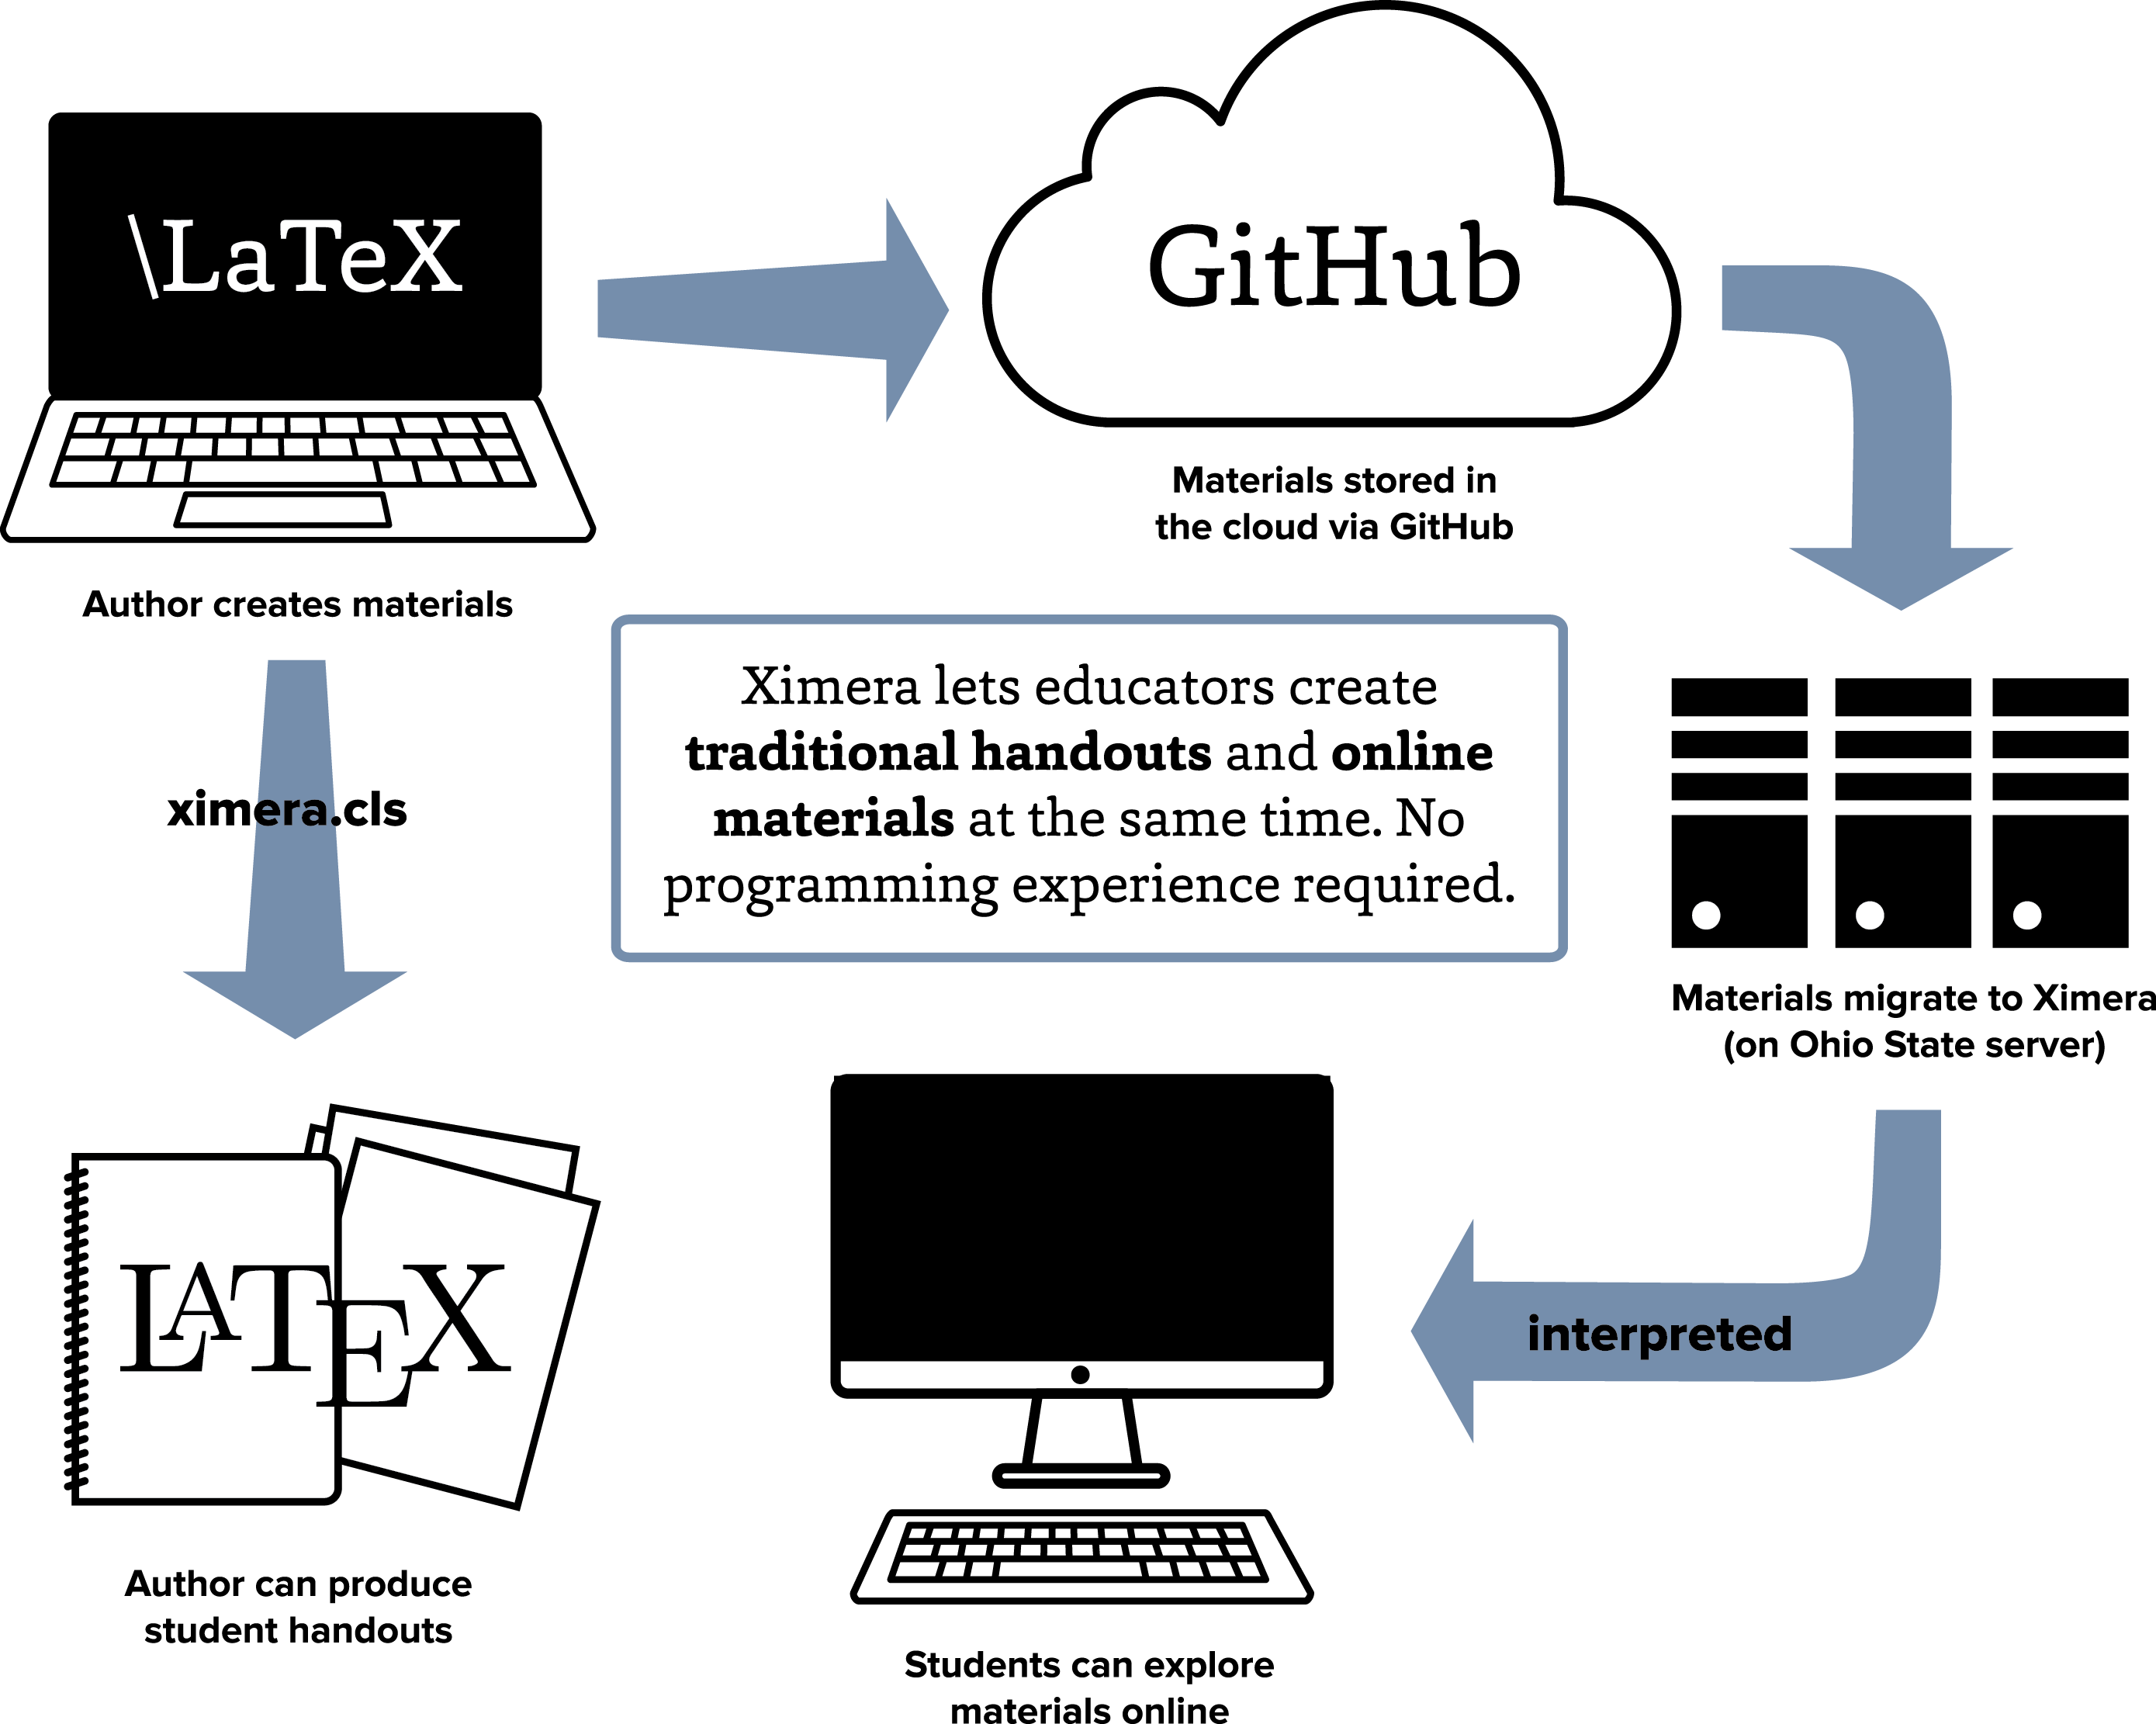
\includegraphics[scale=.25]{XimeraGraphic.png}
\end{image}

One benefit of \href{http://ximera.osu.edu}{\sf Ximera}
is that it provides an easy way to produce interactive online materials.
Another benefit is that many educators, particularly mathematicians,
are already quite familiar with \LaTeX\ and
even find it quite easy to use.
And because the \TeX\ language is extremely static in comparison with
other programming and markup languages, authors can expect
the materials they create to be usable in some
form for the foreseeable future.

\end{document}
